\section{Post-Processing}
\label{sec:pl-postproc}
    % This section discusses the post-processing techniques available in the `MozzPy' package, specifics of the techniques in relation to mosquito detection are explored in section \ref{sec:exp-postproc}.
    \subsection{Filtering}
    \label{subsec:pl-postproc-filt}
        \begin{figure}[ht]
            \centering
            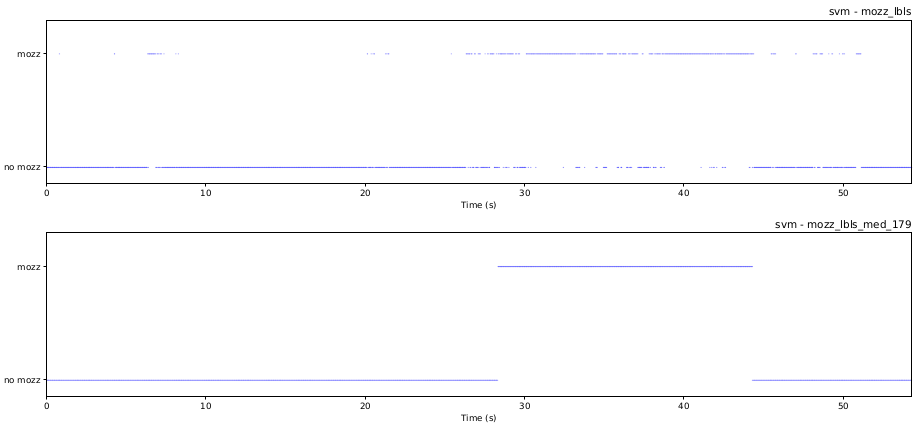
\includegraphics[width=0.9\textwidth]{clfoutput}
            \caption{Raw output of an SVM classifier (above) and median filtered output using a kernel of size $279$ samples or \SI{34.9}{\milli\second} (below).}
            \label{fig:epl-postproc-filt-output}
        \end{figure}
        Because predictions are made on a sample-by-sample basis, results are contain high levels of noise. This is not the way a human makes estimates, rather they label over much longer periods due to the prior knowledge that the mosquito exists in physical space and must travel in and out of range of the microphone. From this prior it can be inferred that a $0$ prediction is much more likely to be preceded by $0$s, and a $1$ prediction will be much more likely to be preceded by $1$s; it is only the edge cases of the pulses where this is not true. 
        
        This prior can be exploited in the form of a moving average filter. A simple rolling median filter could be applied over the output predictions, essentially taking the a majority vote at each window as it rolls across the signal, but then the probabilities associated with the predictions are disjointed, meaning rejection can no longer be applied and metrics that require probabilities are unable to be calculated. Instead, a moving average filter is applied over the probabilities and the labels are recalculated by thresholding at a decision boundary of $0.5$. An example SVM output is shown in Figure \ref {fig:epl-postproc-filt-output}, the effect of the smoothing is clearly depicted where the filtered output is more characteristic of a human label. 
        
        Two filters are implemented, a median filter and a mean filter. The filters are coded to handle $NaN$ values of predictions that have been rejected, where any $NaN$ entries are ignored in the averaging calculation and if all the values are $NaN$ then the output is $NaN$.
        
    \subsection{Asymmetrical Rejection}
    \label{subsec:pl-postproc-rej}
        Rejecting low-confidence classifier outputs was first introduced by \textcite{Chow1970}, only recently has it been explored in depth \cite{SajjadAhmedNadeem,Condessa2017}. Rejection is an emerging field of research and has been applied in contexts such as biomedical imaging, optical character recognition and scene identification \cite{Condessa2017}. The reject option is helpful in two cases, one where the sample does not belong to any class (distance rejection) and the other when the sample is very close to the decision boundary (confusion rejection). In the context of mosquito detection, distance rejection does not apply as all samples belong to either the `no mosquito' or `mosquito' class. This report extends on previous work and introduces asymmetrical rejection, outlined in algorithm \ref{code:pl-postproc-rej}.
        \begin{listing}[ht]
            \begin{minted}[frame=single,framesep=2mm, bgcolor=black!2, fontsize=\footnotesize, linenos]{python}
def apply_rejection(probs):
    res = []
    for prob in probs:
        if (prob > 0.5 and prob > c2_thresh):   # if sample in class 2 & is above class 2 thresh
            res.append(prob)                    # keep it
        elif (prob <= 0.5 and prob > c1_thresh) # if sample in class 1 & is above class 1 thresh
            res.append(prob)                    # keep it
        else:
            res.append(float('nan'))            # reject it
        return res
            \end{minted}
            \caption{Asymmertical rejection algorithm.}
            \label{code:pl-postproc-rej}
        \end{listing} 
        Existing research rejects based a single threshold, here rejection will be determined by two thresholds, one for each class. This is beneficial for cases where the classifier may be better at predicting one class over another so, for example, if the classifier performs well at predicting mosquito presence but poorly in determining when there is not a mosquito, i.e. high true positive rate and low true negative rate, then more aggressive rejection can be applied to the `no mosquito' class predictions without affecting the positive classification performance.
        
    \subsection{Software Implementation}
    \label{subsec:pl-postproc-software}
        Post-processors, as well as being modular, can also be chained. For example, the predictions can first be median filtered then rejection can be applied. All classifier outputs must first go through the \code{get\_mozz\_lblsprobs} post-processer before being further processed or tested. This is to standardise results from arrays, where probabilities are given for each class, to a number, the probability of there being a mosquito. This also handles multi-class results and converts them to a binary output. Results are stored in the same dictionary as the classifier outputs and any test may be applied, discussed in section \ref{sec:pl-test}.
        % \begin{sitemize}
        %     \item{can chain postprocessors in any way}
        %     \item{two more within software: get\_mozz\_probs and get\_mozz\_lbls, applied to all results to make same format}
        %     \item{converts single class/multiclass probability array output into 1d array of probabilities that there is a mozz - useful for further processing and testing}
        %     \item{stores processed results at same level as clssifier output results so can be stored side by side}
        % \end{sitemize} 
